\section{Methodology}
\label{sec:method}
\label{sec:eval:method}% alias: the former Evaluation subsection

\subsection{Hardware Platforms}
The mobile platform pairs the Snapdragon 8 Gen 3~\cite{sd8g3} host and NPU with PIM on LP-Spec's~\cite{lpspec} x64
LPDDR5-6400 (4 dies $\times$ 16 banks, 409.6\,GB/s internal). The NPU computes at 12\,TOPS, its measured FP16 GEMM rate~\cite{hao2025}
used for INT8\ASSUMPTION, and reads the memory at 42\,GB/s (Section~\ref{sec:bg:roofline}). Each host visit costs
30\,\textmu s of NPU dispatch~\cite{npufaster}\ASSUMPTION; the host draws 2.285\,W while busy, the 8 Gen 3's~\cite{sd8g3}
decode power net of its DRAM~\cite{hao2025,heterollm,tman}\ASSUMPTION. The edge server pairs P3-LLM's~\cite{p3llm} NPU with one
HBM2 stack of 16 pseudo-channels (1,024\,GB/s internal); the NPU idles at 55\,W, the chip idle power of
TPUv4i~\cite{tpuv4i}, while the PIM works\ASSUMPTION.

\subsection{PIM Designs and Area}
Each substrate carries four designs, stock AiM~\cite{aimjssc}, P3-LLM-style, LP-Spec-style and CoDe, with one
controller and the same PU placement (Table~\ref{tab:params}). Every design computes at its rival's
precision: INT8 on the mobile platform, as LP-Spec~\cite{lpspec} does, and W4A8 with a 4-bit KV cache on HBM2, as
P3-LLM~\cite{p3llm} does, with every design's arithmetic priced as INT4\,$\times$\,INT8 integers\ASSUMPTION. On the
mobile platform CoDe's tile of $V = 8$ spans two column periods, so one MAC command serves eight tokens. On HBM2 each
token's staging slice is twice as large and every PU serves two banks, so CoDe uses $V = D = 4$
there; Section~\ref{sec:eval:ablation} sizes $V$ on both platforms. CoDe reaches LP-Spec-style's peak on
the mobile platform with 0.539$\times$ its logic area per die: arithmetic takes 0.73 of LP-Spec-style's logic and 0.34
of CoDe's, while storage, the staging queue, accumulator file and weight latch, takes 0.32 of CoDe's logic and 0.10
of LP-Spec-style's. On HBM2, CoDe's logic is 0.56$\times$ LP-Spec-style's and 1.33$\times$ P3-LLM-style's, an area
that buys twice P3-LLM-style's beats per column.

\subsection{Simulator and Models}
% figure* (Section VI-A): defined at V-C's start (page 8), so it renders at the top of the next page, where VI-A cites it
\begin{figure*}[t]
  \centering
  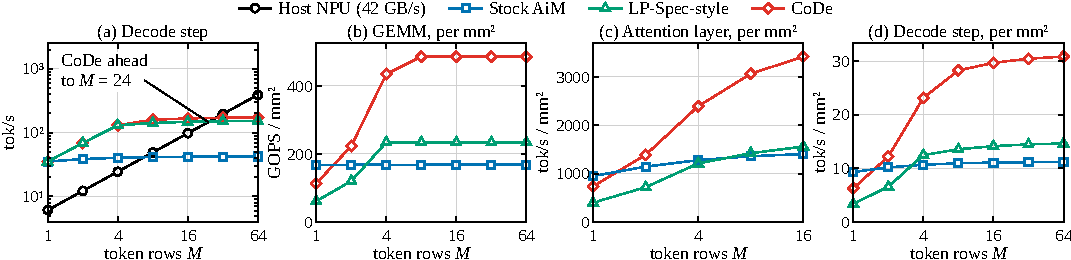
\includegraphics[width=\textwidth]{figs/fig_phone.pdf}
  \caption{Mobile platform: (a)~decode-step speed; (b)~GEMM, (c)~attention-layer and (d)~decode-step throughput per
  logic mm$^2$.}
  \label{fig:phone}
\end{figure*}

We extend the open-source trace-driven AiM simulator, built on Ramulator~2.0~\cite{ramulator2} and used by
CENT~\cite{cent}, with each design's commands and a PU model that holds a MAC command until the PU has finished the
beats of the previous command; every PIM kernel runs at cycle level. Our P3-LLM-style model reproduces
P3-LLM's~\cite{p3llm} own step gain of depth 2 over a depth-1 PIM: 1.78$\times$ at INT8 against the 1.6$\times$ P3-LLM
reports. On the mobile platform the simulator gives P3-LLM-style's per-token commands no separate C/A slot;
re-timed on the C/A bus, the commands lower P3-LLM-style's $U$ from 0.384 to 0.380, and on the edge server the
simulator times them. The mobile runs issue refreshes without their refresh cycle time, so refresh takes no share of
the mobile time ($\rho = 0$ in Section~\ref{sec:bg:cmd}). Area comes from synthesis of each PU's lanes and registers in a 45\,nm library, scaled to a 1z DRAM process by
the published area of AttAcc's~\cite{attacc} GEMV unit in that process; the GB is priced as DRAM-process
SRAM\ASSUMPTION. PU power and energy come from synthesis of each design's whole PU with Yosys and ABC~\cite{abc} on the
Nangate45 library, OpenROAD~\cite{openroad} placement and clock-tree synthesis, and OpenSTA power from a zero-delay
simulation with random operands. We scale the synthesised energy to the DRAM process so that an AiM-style bf16 PU from
the same flow spends the compute share of CENT's~\cite{cent} AiM MAC-command energy, and with the square of the voltage
to the 1.05\,V supply (VDD2H on LPDDR5); leakage scales the same way\ASSUMPTION. Peak power runs every PU at its full
MAC rate and includes leakage, GB reads and the column fetch, which adds 87.6\,mW per die on the mobile platform and
54.8\,mW per pseudo-channel on HBM2 to every design. Energy per token charges each issued MAC its PU's synthesised energy,
leakage over the step time, GB reads priced by SRAM size~\cite{horowitz}, and CENT's~\cite{cent} per-command DRAM
energies. In every design a PU's clock runs only on its MAC beats, so an idle PU cycle costs leakage
only\ASSUMPTION.

\subsection{Algorithms and Workloads}
The mobile platform runs speculative decoding of Llama-2-7B in INT8 with a 1.1B-parameter draft model or an EAGLE
head~\cite{eagle}: $M - 1$ drafted tokens and one verify pass of $M$ rows, acceptance rate 0.7 per token, context
$L = 128$--1024, and each design at its fastest $M$. GEMMs use six FC shapes of Llama-2-7B and Llama-3.2-1B, and attention layers use three head configurations at $L = 128$--4096. The edge server runs batched decoding of Llama-2-7B
and 13B, Llama-3.1-8B, Llama-3.2-3B and Mistral-7B at a 4K context, batch $M = 1$--64, one token per request per step.

\subsection{Metrics}
Speed is tokens per second, end to end or of one decode step; area efficiency is that throughput per mm$^2$ of PIM
logic, over all four dies or all 16 pseudo-channels; energy is system energy per token. On HBM2 one all-bank column counts as one command and as two half-column slots in the C-bus occupancy. Ranges on the mobile platform span every $M$ and $L$; ranges on the edge server are the minimum and maximum of per-$M$ geometric means over the five models.
